\chapter{Architecture}
\label{chapter:architecture}
Esta secção deve englobar:

\begin{itemize}
    \item Uma análise de requisitos, onde devem “abrir” portas para as principais
        características da vossa arquitectura.
    \item Uma descrição de alto nível da arquitectura do vosso sistema. Esta descrição
        pode ser:
        \begin{itemize}
            \item A arquitectura de rede, explicando os principais componentes e as
                funções que executam.
            \item A arquitectura de SW da aplicação, explicando os principais
                componentes e as funções que executam.
        \end{itemize}
    \item Descrições detalhadas de todos os componentes da vossa arquitectura.
    \item As escolhas que efectuarem em termos de arquitectura global e de detalhe,
        devem ser justificadas, face aos requisitos que identificaram.
\end{itemize}

Sempre que possível, ilustrem a arquitectura com figuras, que descrevam
sucintamente o modelo como na Figure~\ref{fig:logoCNM}.

\begin{figure}[!htb]
  \centering
  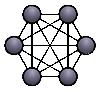
\includegraphics[width=0.25\textwidth]{Figures/logoCNM.png}
  \caption[Caption for figure in TOC]{Caption for figure.}
  \label{fig:logoCNM}
\end{figure}



This section describes the architecture of the system, a platform for office automation and security designed to offer greater comfort to the occupants, reduce the energy use with minimum intervention and intrusion detection.

This section is divided in four subsections: \ref{architecture1} starts by defining the requirements of the system that will lead the design of our architecture. In Section \ref{architecture2} the architecture of the system is described. Finally, Section \ref{architecture3} and \ref{architecture4} present a brief overview of the hardware and software architectures.

%This chapter is divided in four sections: Section 3.1 starts by defining the requirements of the system
%that will lead the design of our architecture. In Section 3.2 the architecture of the system is described in
%depth. Finally, section 3.3 and 3.4 present a brief overview of the hardware and software architectures



\subsection{System Requirements}\label{architecture1} 

In order to choose the appropriate architecture in terms of performance, functionality, extensibility and comfort, the system must satisfy the following set of requirements:

\begin{itemize}
  \item \textbf{Scalable:} The system must be scalable and offer rapid deployment of new nodes.
  \item \textbf{Isolation:} The control and automation of the offices must be independent and work regardless the state of the rest of the system.
  \item \textbf{Multiuser:} The system must be able to maintain multiple user preferences, in the eventuality of multiple users occupying the room at the same time the system must be capable of adjusting the ambient settings to minimize their discomfort. 
  \item \textbf{Manual control:} People expect to be some form of manual control over the room such a light switch or thermostat, the system must provide a graphical interface embedded in the wall that allows manual control of some basic services such as HVAC and lighting.
  
  \item \textbf{Remote control:} It should provide a authenticated user status and remote control over the room's services, by the use of an Android app.
  \item \textbf{Automate tasks:} The user should be able to configure tasks to be triggered by a scheduler or sensor value.
  \item \textbf{Load-aware:} The system must be able to adjust services such as HVAC and lighting in a energy efficient way.
  \item \textbf{Human aware:} It must be capable of detecting human presence inside the room with high certainty.
  \item \textbf{User aware:} It must capable of detecting if the user is inside the building with a medium/low accuracy and the user presence in the room with high Accuracy
  \item \textbf{Energy Efficient:} The system must be able to adjust it's own energy footprint during long periods when no occupant is within the room, such as nigh time.  
  
\end{itemize}




\subsection{Architecture Overview}\label{architecture2} 




The proposed system consists of three main components: the User App, the HUB and Zone Controller. The User App allows remote control over the HUB services as well as provides the HUB with user location data. The HUB is responsible for the room automation and security systems, collection of sensor data and manual control over the room services. The Zone Controller functions as a HUB but it can also communicate with the HUBs and be alerted to changes in the rooms (zones), because its at the top of the hierarchy it will perform tasks relevant to the entire building zone.

As represented in Figure \ref{architecture_system}, every HUB is able to work without the presence of the Zone Controller or any User App. Several smart-phones with the User App are able to interact with the HUB. The same way, the Zone Controller can connect to one or more HUBs.

In the next sections we will detail the three main components of the system.

\begin{figure}[h]
\centering
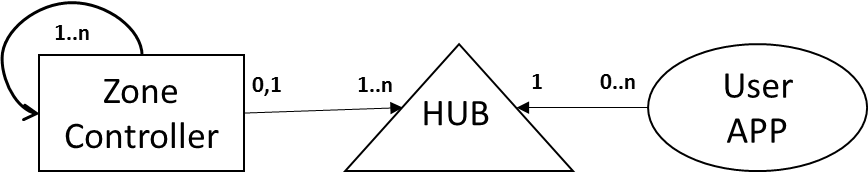
\includegraphics[width=0.7\textwidth]{Figures/architecture}
\caption{Architecture of the system}
\label{architecture_system}
\end{figure}


\subsubsection{User App}\mbox{}\\

The User App running in the users mobile devices offers remote control over the office services and security as well as provide the HUB with user recognition and location data. The User App will notify the HUB of the user presence inside the building and help to identify the user within the room itself.



\subsubsection{HUB}\mbox{}\\

The HUB, will be present in every office, it is the most important component of the system. It is responsible for controlling the HVAC and electrical devices of the office, enforcing energy saving policies, improve occupant comfort and provide security monitoring during the hours when the user is away from the office.
It will feature an user interface for manual control over the services provided.

\textbf{HUB communication} with the Zone Controller or the User App will be done using Wi-Fi networks. When inside the building the pre-installed wireless network will be used to enable communication between all components, when outside the building a connection with internet access can be used to remote control the HUB. The HUB can also communicate with external devices using Bluetooth or Bluetooth Low Energy.


\subsubsection{Zone Controller}\mbox{}\\

The Zone Controller component has all the functionalities of the HUB. It can also communicate with several HUBs and gather on-demand data from them. This component will be responsible for services that are common to the whole building.

The goal of the Zone Controller is to take certain actions based on collected information from the HUBs, for instance when all the offices in a corridor are empty then the corridor lights can be turned off or dimmed. If several Hubs try to use the building HVAC and the boilers are turned off, then a Zone Controller installed at the boiler could turn it on. 

To protect the privacy of office occupants, video streaming monitoring service will not be shared by the HUBs with the Zone Controller.

The system can be deployed in just a room, if cooperation is not required, in that case the Zone Controller is not needed and the system can work with just the HUB.



\subsection{Hardware Architecture}\label{architecture3} 

The HUB has two main hardware components, one is the Android tablet that provides the sensors, the connectivity, the storage as well as a camera, microphone, speaker and a touch screen. 
The other component is the microcontroller, it allows the digital world to interact with the real world through the use of actuators that convert electric signal into mechanical actions. The microcontroller is connected to the actuators (relay) and is able to switch on/off the lights as well as controlling the HVAC. This component is needed because typically lights and HVAC system don't have any type of connectivity other than the electric wires. 


If the room had installed wireless devices that communicate with technologies such as ZigBee or Z-Wave then the microcontroller could be connected to a radio module able to communicate with those wireless technologies such as a xbee module.

%Besides the above hardware requirements 

Figure \ref{architecture_system}, represents a HUB, its components and the main communication protocols used.

 

\subsubsection{Communication Protocols}\mbox{}\\

The system requires that all the three components: Zone Controller, HUB and User App, are able to communicate. The three components will use Wi-Fi to communicate data at high data rate, the HUB and the User App can also use Bluetooth Low Energy to determine if the two are close to each other. Likewise the HUB can use BLE to communicate with external sensors. The communication between the Android tablet and the microcontroller is done using a micro-B USB cable using serial communication. Finally the communication among the microcontroller and the actuators is done by using the General Purpose Input/Output (GPIO) pins.




\begin{figure}[h]
\centering
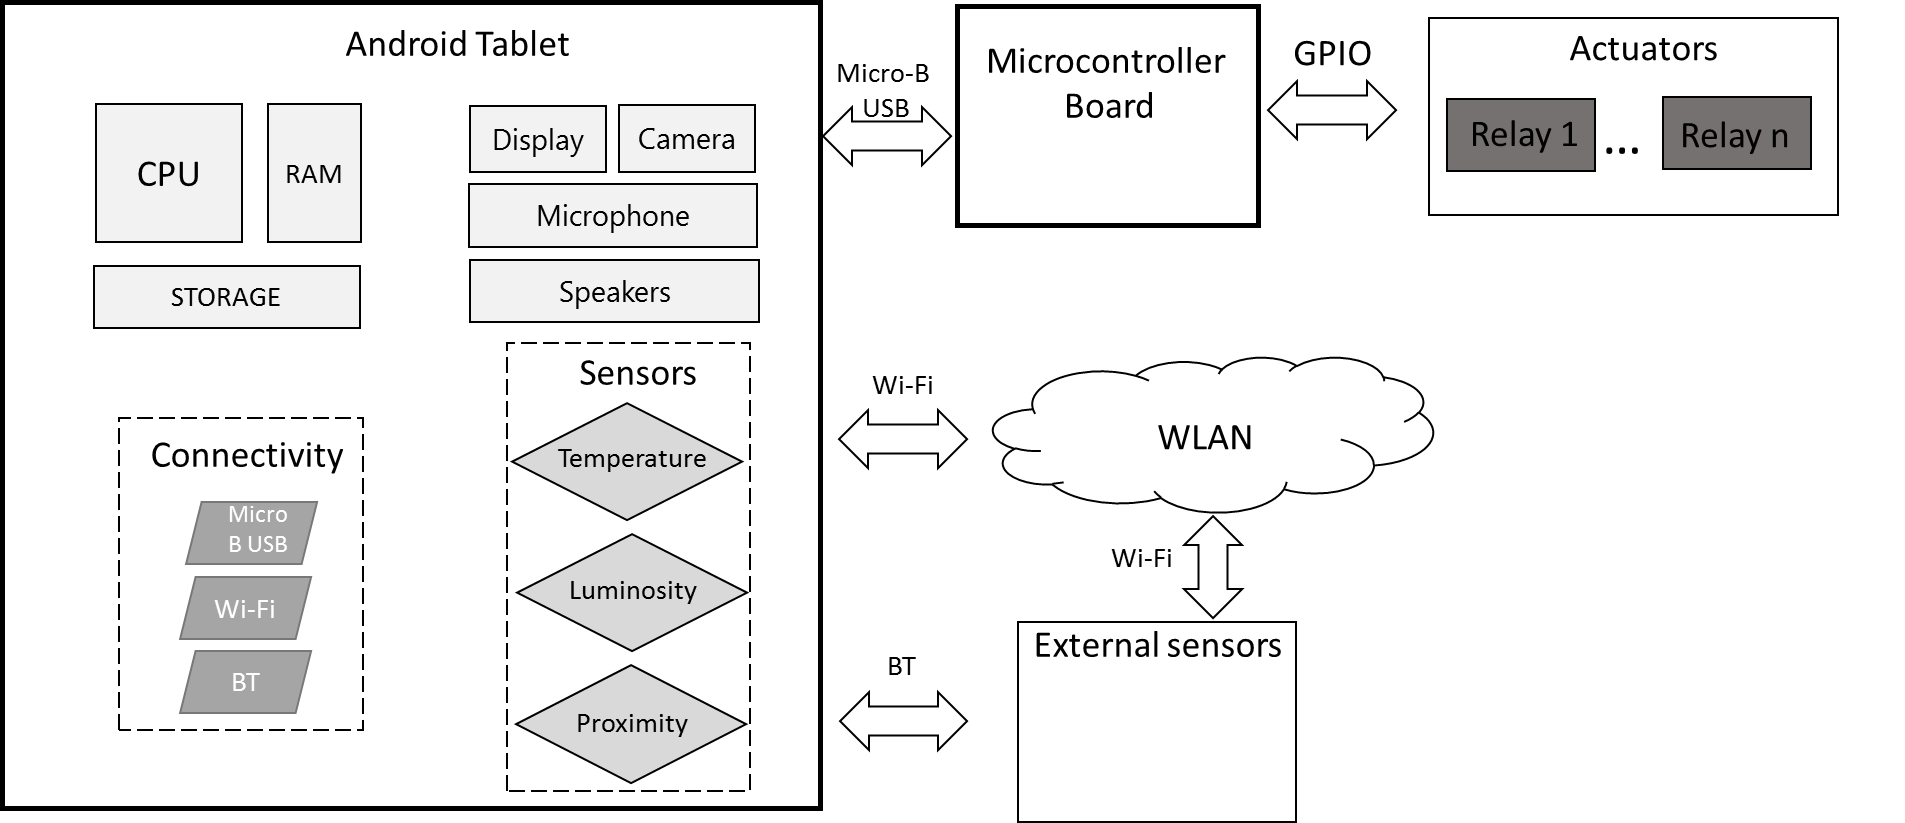
\includegraphics[width=0.9\textwidth]{Figures/hardware}
\caption{Hardware architecture of the HUB}
\label{architecture_system}
\end{figure}


\subsection{Software Architecture}\label{architecture4} 


There will two Android APPs in the system, one will be the HUB APP that runs in the tablets mounted in the rooms. The other is the User APP that the occupant of the room can install to remote control the HUB, allow user recognition and video monitoring of the room. 

Figure \ref{software1}, describes a top view over the system. Both Apps will communicate over WLAN and Bluetooth with each other. Bluetooth communication will be in the form of BLE beacon, where the HUB will act as a beacon and when the user app detects this beacon it will notify  the HUB of its proximity helping with user detection. Wi-Fi will be used to transfer application data, the JavaScript Object Notation (JSON) standard will be used as the message format. JSON was chosen as there are libraries capable of converting java object models into JSON, allowing for simple transfer of java models between different Android devices. This also means that in the future our system could communicate with other devices and interoperate by using JSON, as long as the other device knows the types of messages supported by our system.

The Android tablet will connect to the microcontroller through the use of an USB On-The-Go (OTG) cable. With a normal USB cable the Android tablet would not be able to communicate since it can only be a client. USB OTG allows the devices to switch the roles of client and host enabling the android tablet to communicate with the microcontroller. Messages can be sent using Serial communication and are received one character at a time by the microcontroller.

Communication to external sensors will use BLE and follow the application programming interface (API) specified by those devices.






\begin{figure}[h]
\centering
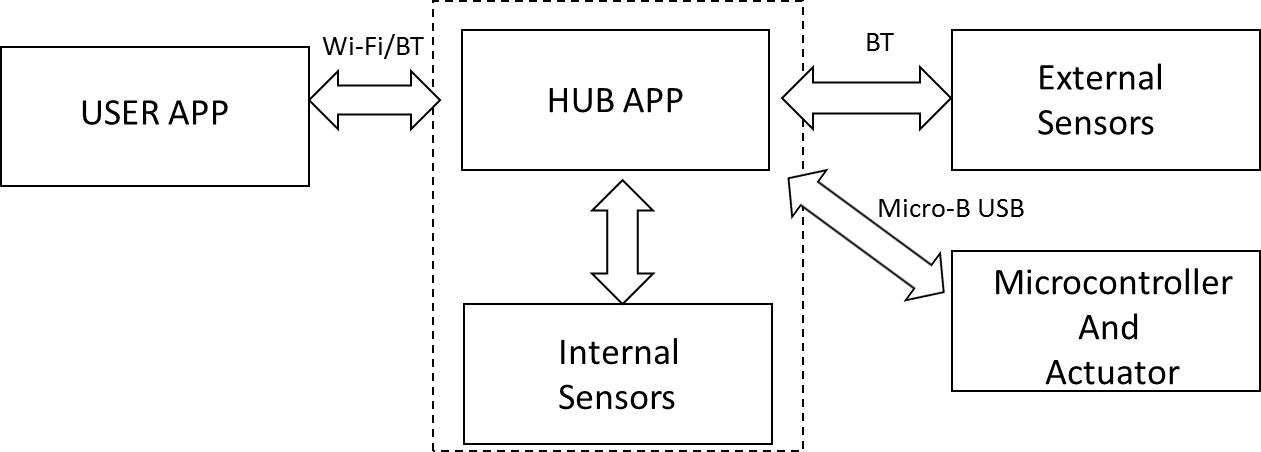
\includegraphics[width=0.9\textwidth]{Figures/software1}
\caption{Software architecture of the system}
\label{software1}
\end{figure}


In order to provide higher comfort and user detection, our system requires that both the user and the HUB have installed an app. Since the requirements for the User App and the HUB App are different in many aspects two architectures are proposed. These different functionality requirements are due to the nature that the HUB has to operate a automation and security system. Yet the user app only needs to send and receive data.
\subsubsection{HUB App Architecture}\mbox{}\\

The presented architecture is designed to run in the HUB, several managers are proposed. Figure \ref{software2}, represents the the architecture of the HUB App.

\paragraph{User Interface}\mbox{}\\
This is the interface seen in the HUB screen, it will offer:

\begin{itemize}
  \item Manual control of the lighting and HVAC systems.
  \item User registration, QR Code association.
  \item User identification, if no User App is available an unique QR Code can be used as authentication.
  \item Real-time ambient sensors readings.
  \item Security settings, enable/disable security monitoring and notification email.
  \item General settings, activate voice control, allow sound.
   
\end{itemize}

\paragraph{Automation Manager}\mbox{}\\
The Automation Manager is responsible for controlling the automation logic, we can only interact with the lighting and HVAC systems through it. It also has a scheduler responsible for executing repetitive tasks at regular time intervals or at fixed moments. It is also possible to create IFTTT rules. The Automation Manager will check if the condition for the rule has been satisfied and trigger the action.


\paragraph{Security Manager}\mbox{}\\
It is responsible for occupant detection inside the room, by using the camera to detect changes that would indicate motion, as well as other data such as the opening and closing of the door and the user location received from the User Location Manager.

This manager is responsible for user authentication and permission cheeking of requests made by the mobile user app to the HUB.


\paragraph{User Location Manager}\mbox{}\\
The User Location Manager tracks the whereabouts of the user inside the building, in association with the User APP, it is notified when the user enter the building. It also controls a BLE beacon service that enables the User App to know the distance to the beacon in order to notify the Location manager of this proximity.

\paragraph{Storage Manager}\mbox{}\\
The Storage Manager is responsible for saving and retrieving the application data, the data can be saved in several different storage option: SharedPreferences, SQLite, disk file.

\paragraph{User Manager}\mbox{}\\
User Manager keeps the user preferences and user associated authentication token. It is also responsible for registering new users and generating unique QR Codes that act as a identification token.

\paragraph{Sensor Manager}\mbox{}\\
Sensor Manager allows access to the tablet's sensors as well as the external sensors. It abstracts external sensors into virtual sensors.


\paragraph{Communication Manager}\mbox{}\\
The Communication Manager allows the abstraction of the communication layer between the tablet and the outside components, it will offer:

\begin{itemize}
  \item HTTP Server thread, it receives and sends JSON messages to the user app. The received messages are routed to the manager specified in the message.
  \item Email notification with alerts, triggered by the Security Manager.
\end{itemize}

\paragraph{Environment Interaction Manager}\mbox{}\\
The Environment Interaction Manager will abstract every actuator connected to the microcontroller allowing them to be treated as virtual devices. Every virtual device is defined as a stateful object that reflects the present state of a physical device. Since the devices represent actuators they are Readable and Writable.

\begin{figure}[h]
\centering
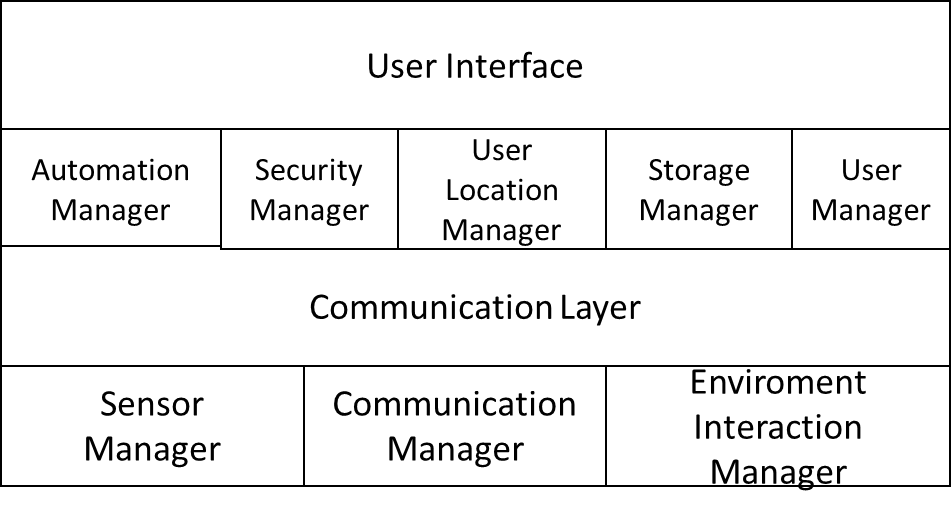
\includegraphics[width=0.6\textwidth]{Figures/software2}
\caption{HUB APP architecture }
\label{software2}
\end{figure}



\subsubsection{User App Architecture}\mbox{}\\
The User App is simpler than the HUB App, several managers were suppressed. Figure \ref{software3}, represents the the architecture of the User App.

\paragraph{Control Manager}\mbox{}\\
The Control Manger offers remote control over the HUB's services. It uses AsyncTask to asynchronously communicate. The manager can control the state of the lighting and HVAC systems, as well as read the sensors values from the HUB's Automation Manager and Sensor Manager .
It can communicate with the HUB's Automation Manager to create IFTTT rules and use the Security Manager to enable monitoring and view the camera video stream. 

\paragraph{User Location Manager}\mbox{}\\
It cooperates with the HUB to allow the tracking of the user location. There is a service that runs in the background that checks the visible wireless networks SSID, if the network associated with the building is found it communicates with the HUB every 10 minutes. This regular check allows the HUB to know if the user has left the building, if the user was in the building and no check is received then the user is most likely outside the building. 
An other background service also scans for BLE beacons, if the Universally unique identifier (UUID) associated to the HUB's beacon is found it communicates with the HUB. Regular checks will also be used to determine if the user is still in the office. The interval between checks will be further studied in order to provide adequate time between scans and be conservative regarding the user's mobile device battery.

\paragraph{Storage Manager}\mbox{}\\
The User App Storage Manager is the same as the HUB's Storage Manager.


\paragraph{User Manager}\mbox{}\\
The User Manager keeps the token used to authenticate the user. It also enables registration in the system. In order to register a new user the occupant must select the registration option in the HUB's screen. A QR Code will be generated, the user must point the phone camera at the QR Code and the app will register the new user. If the user does not have an Android phone with the User App installed it is also possible to take a picture of the QR Code and manually register the user in the HUB. The picture of the QR Code will authenticate the user if he does not have the User App installed. The  user needs to select the manual authentication option in the HUB and show the QR Code image to the camera of the HUB.

\paragraph{Communication Manager}\mbox{}\\
It offers the other Managers with an AsyncTask message sending service, the messages are sent in JSON format.

\begin{figure}[h]
\centering
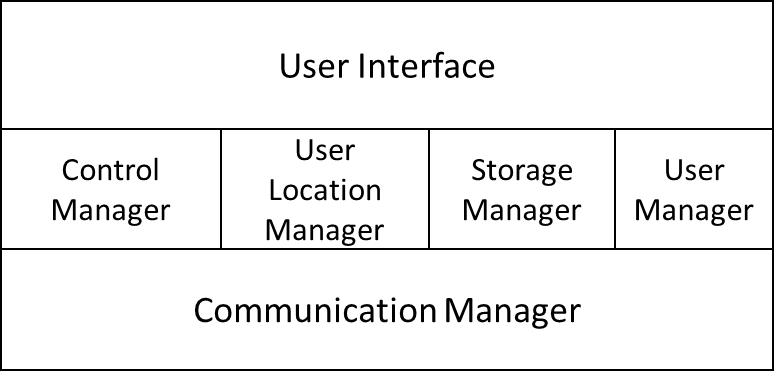
\includegraphics[width=0.5\textwidth]{Figures/software3}
\caption{User APP architecture }
\label{software3}
\end{figure}
